\section{DIP开发者激励协议}
\label{sec:dip}

\subsection{设计目标}
\label{dip:design}
为了更好地建立区块链应用的生态环境,在星云链中,我们提出面向智能合约开发者的DIP(Developer Incentive Protocol,开发者激励协议),通过星云币的奖励来感谢为生态助力的优秀智能合约开发者。

\subsection{DIP奖励分配算法}
\label{dip:arith}
我们认为,一个智能合约是否优秀取决于有多少用户愿意使用它,而且有更多的高价值账户使用的智能合约更加优秀,而作为账户普适价值尺度的NR正好可以应用在高价值账户的评估中。DIP的设计结合NR和常用的周活跃用户的概念,使用周活跃用户的价值尺度总和来衡量智能合约的价值尺度,然后使用该价值尺度来评估开发者的贡献度。

DIP按周期进行一次,和Nebulas Rank计算周期一致。对于智能合约C,假设本周活跃账户地址集合为WAA(Weekly Active Addresses),其中根据\refsec{subsec:leaderrank}的NR排名(取Top X,值为1-X),计算周活跃地址的NR之和作为合约C的贡献度SCS(Smart Contract Score),如公式\ref{formula:dip:scs}。

\begin{align}
\label{formula:dip:scs}
SCS(C)=\sum_{addr \in WAA}(max\{X + 1 - NR(addr), 0\})
\end{align}

按照每周贡献值SCS从高到低排序得到智能合约贡献度排名SCR(Smart Contract Rank),取Top N的智能合约,它们对应的开发者将按比例瓜分M个星云币作为奖励,为了避免恶意刷榜,DIP的分配曲线被设计得较为平均,如图\ref{fig:dipdis}所示,但依旧保证Rank 1的收益为Rank N收益的一倍以示贡献度大小的区别,比例约束见公式\ref{formula:dip}。

\begin{alignat}{2}
Coin(C) = & \quad kln(N+1-SCR(C))+b \label{formula:dip} \\
\mbox{s.t.}\quad & kln(N) + b = 2b \nonumber \\
& \sum_{x=1}^{N}(kln(x) + b) = M \nonumber
\end{alignat}

\begin{figure}[h]
\centering
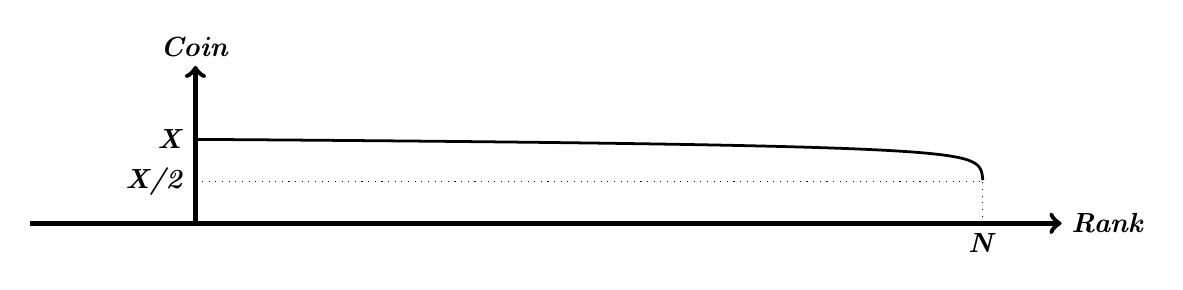
\begin{tikzpicture}
\coordinate (OR) at (0.00, 0.00);
\coordinate (LX) at (-2.10, 0.00); % left x
\coordinate (RX) at (11.00, 0.00); % right x
\coordinate (BY) at (0.00, 0.00); % bottom y
\coordinate (TY) at (0.00, 2.00); % top y
\draw[->][line width=1.75pt] (LX) -- (RX);
\node[right,black] at (11,0) {\textbf{\textit{Rank}}};
\draw[->][line width=1.75pt] (BY) -- (TY);
\node[above,black] at (0, 2) {\textbf{\textit{Coin}}};
\draw[dotted] (0,0.533210267)--(10,0.533210267);
\draw[dotted] (10,0)--(10,0.533210267);
\node[below,black] at (10, 0) {\textbf{\textit{N}}};
\node[left,black] at (0, 0.533210267) {\textbf{\textit{X/2}}};
\node[left,black] at (0, 1.066420536) {\textbf{\textit{X}}};
\draw[black, line width=1.00pt, domain=0:10.00,samples=3000] plot[smooth](\x, {.066598275 * ln(3001-\x * 300) + .533210267});
\end{tikzpicture}
\caption{DIP奖励分配曲线}
\label{fig:dipdis}
\end{figure}

DIP的奖励将会由各个节点单独计算发放,假设星云链平均每S秒出一个区块,那么每隔24*7*3600/S个区块,所有节点将会计算一次DIP的奖励,并且发给对应的智能合约的提币地址中。

为了鼓励星云链生态智能合约的多样性,让更多新生开发者的优秀成果也能获得激励,DIP规定每个智能合约最多可以接受K次奖励。DIP将会根据排名每次选出还可以接受奖励的Top N智能合约给予激励,助推区块链应用生态发展。

\subsection{实验结果}
\label{dip:economic}

我们收集了以太坊上从2017年5月份交易数据,计算了第一周的DIP排名,如表\ref{table:dip}所示。

\begin{table}[h]
\centering
\begin{threeparttable}[b]
\caption{2017年5月第一周\tnote{1}DIP排名结果Top 10}
\label{table:dip}
\begin{tabular}{ccc} \toprule
    {Contract~Address} & {Score} & {Description\tnote{2}} \\ \midrule
0xa74476443119a942de498590fe1f2454d7d4ac0d & 264456363.0 & GolemToken \\
0x49edf201c1e139282643d5e7c6fb0c7219ad1db7 & 207900181.0 & TokenCard-ICO \\
0x48c80f1f4d53d5951e5d5438b54cba84f29f32a5 & 129625776.0 & REP-Augur-OLD \\
0x6810e776880c02933d47db1b9fc05908e5386b96 & 108324489.0 & Gnosis-TokenContract \\
0x6090a6e47849629b7245dfa1ca21d94cd15878ef & 54429341.0 & ENS-Registrar \\
0x607f4c5bb672230e8672085532f7e901544a7375 & 48526808.0 & RLC \\
0x8d12a197cb00d4747a1fe03395095ce2a5cc6819 & 46498412.0 & etherdelta\_2 \\
0xf7b098298f7c69fc14610bf71d5e02c60792894c & 43746158.0 & GUPToken \\
0xaaaf91d9b90df800df4f55c205fd6989c977e73a & 42026627.0 & TokenCardContract \\
0xaec2e87e0a235266d9c5adc9deb4b2e29b54d009 & 41427314.0 & singularDTVToken \\
\bottomrule                                                     
\end{tabular}	
\begin{tablenotes}
  \small
  \item[1] 区块范围[3629091, 3665815]
  \item[2] 来自etherscan.io
\end{tablenotes}
\end{threeparttable}
\end{table}

可见,DIP排名靠前的合约较为知名,在计算周期内也更为活跃,符合我们激励生态建设者的初衷。

\subsection{作弊分析}
\label{dip:sybil}

智能合约只能被动调用,不能主动和非合约账户建立交易,所以一个作弊者想要让他的智能合约排名上升,就必须要找到足够多的高NR排名账户来调用他的合约。

首先,作弊者想要零成本提升DIP排名将不可能实现。假设作弊者想要提高合约C的排名,并为此伪造了大量账户,但由于在公式\ref{formula:dip:scs}中计算SCS时,只有NR排名中Top X的调用贡献分大于0,新伪造出来的账户NR排名将会在Top X之外,即使调用合约C也对DIP的排名没有任何影响。

其次,如果作弊者愿意为合约的DIP排名上升付出一定的成本,那么他有两种方式可以选择。第一种,自己花钱伪造高NR的账户来调用合约C,提升合约C的排名。而要伪造高NR的账户在\refsec{subsec:robust}已有分析,每提升一个账户都需要投入一大笔资金来伪造该账户特殊的拓扑结构,并且由于NR的周期性更新,长期维持高NR的成本将会巨大。第二种,作弊者找到大量高NR账户,说服或者贿赂他们来调用合约C,这种链下行为难以规模化,作弊者花了很大精力找到的高NR账户也只会占Top X中的一小部分,对真正优秀的合约影响不大。

